\documentclass[12pt, letterpaper, notitlepage, onecolumn, twoside, openbib]{article}\usepackage[]{graphicx}\usepackage[]{color}
%% maxwidth is the original width if it is less than linewidth
%% otherwise use linewidth (to make sure the graphics do not exceed the margin)
\makeatletter
\def\maxwidth{ %
  \ifdim\Gin@nat@width>\linewidth
    \linewidth
  \else
    \Gin@nat@width
  \fi
}
\makeatother

\definecolor{fgcolor}{rgb}{0.345, 0.345, 0.345}
\newcommand{\hlnum}[1]{\textcolor[rgb]{0.686,0.059,0.569}{#1}}%
\newcommand{\hlstr}[1]{\textcolor[rgb]{0.192,0.494,0.8}{#1}}%
\newcommand{\hlcom}[1]{\textcolor[rgb]{0.678,0.584,0.686}{\textit{#1}}}%
\newcommand{\hlopt}[1]{\textcolor[rgb]{0,0,0}{#1}}%
\newcommand{\hlstd}[1]{\textcolor[rgb]{0.345,0.345,0.345}{#1}}%
\newcommand{\hlkwa}[1]{\textcolor[rgb]{0.161,0.373,0.58}{\textbf{#1}}}%
\newcommand{\hlkwb}[1]{\textcolor[rgb]{0.69,0.353,0.396}{#1}}%
\newcommand{\hlkwc}[1]{\textcolor[rgb]{0.333,0.667,0.333}{#1}}%
\newcommand{\hlkwd}[1]{\textcolor[rgb]{0.737,0.353,0.396}{\textbf{#1}}}%
\let\hlipl\hlkwb

\usepackage{framed}
\makeatletter
\newenvironment{kframe}{%
 \def\at@end@of@kframe{}%
 \ifinner\ifhmode%
  \def\at@end@of@kframe{\end{minipage}}%
  \begin{minipage}{\columnwidth}%
 \fi\fi%
 \def\FrameCommand##1{\hskip\@totalleftmargin \hskip-\fboxsep
 \colorbox{shadecolor}{##1}\hskip-\fboxsep
     % There is no \\@totalrightmargin, so:
     \hskip-\linewidth \hskip-\@totalleftmargin \hskip\columnwidth}%
 \MakeFramed {\advance\hsize-\width
   \@totalleftmargin\z@ \linewidth\hsize
   \@setminipage}}%
 {\par\unskip\endMakeFramed%
 \at@end@of@kframe}
\makeatother

\definecolor{shadecolor}{rgb}{.97, .97, .97}
\definecolor{messagecolor}{rgb}{0, 0, 0}
\definecolor{warningcolor}{rgb}{1, 0, 1}
\definecolor{errorcolor}{rgb}{1, 0, 0}
\newenvironment{knitrout}{}{} % an empty environment to be redefined in TeX

\usepackage{alltt}
\usepackage{amsmath}
\usepackage{amssymb}
\usepackage{amsfonts}
\usepackage{enumerate}
\usepackage{mathrsfs}
\usepackage{verbatim}
\usepackage{float}
\usepackage{turnstile}
\usepackage{epsf,graphicx,psfrag}
\usepackage{rotating, graphicx}
\usepackage{lscape}
\usepackage{latexsym}
\usepackage{epstopdf}
\usepackage{setspace}
\usepackage[top=1in, bottom=1in, right=1in, left=1in]{geometry}
\usepackage{dcolumn}
\usepackage{booktabs}
\usepackage{mathtools}
\usepackage{threeparttable}
\usepackage[labelsep=period,font={bf},textfont={normalsize},labelfont={normalsize}]{caption}


\newcolumntype{.}{D{.}{.}{-1}}      % Allows alignment of decimal places
\newcolumntype{d}[1]{D{.}{.}{#1}}
%\usepackage[style=authoryear]{biblatex}
\usepackage[authoryear,round,longnamesfirst]{natbib}
\usepackage[hidelinks]{hyperref}
\usepackage{apalike}

\doublespacing

%\bibliography{biblioperu}
\usepackage{url}
\usepackage{fancyhdr}
\pagestyle{fancy}
\lhead{}
\chead{}
\rhead{}
\cfoot{ - page \thepage}
\renewcommand{\headrulewidth}{0pt}
\newcolumntype{L}[1]{>{\raggedright\arraybackslash}m{#1}}




\IfFileExists{upquote.sty}{\usepackage{upquote}}{}
\begin{document}


\title{Homework}

\date{ }

\maketitle


\begin{knitrout}
\definecolor{shadecolor}{rgb}{0.969, 0.969, 0.969}\color{fgcolor}\begin{kframe}
\begin{alltt}
\hlkwd{load}\hlstd{(}\hlstr{'nigeria.rda'}\hlstd{)}

\hlstd{years} \hlkwb{=} \hlkwd{sort}\hlstd{(}\hlkwd{unique}\hlstd{(nigeria}\hlopt{$}\hlstd{year))}
\hlstd{groups} \hlkwb{=} \hlkwd{with}\hlstd{(nigeria,} \hlkwd{intersect}\hlstd{(sender, receiver))}
\hlstd{n} \hlkwb{=} \hlkwd{length}\hlstd{(groups)}
\hlstd{adjmat} \hlkwb{=} \hlkwd{matrix}\hlstd{(}\hlnum{0}\hlstd{,}\hlkwc{nrow} \hlstd{= n,} \hlkwc{ncol} \hlstd{= n,} \hlkwc{dimnames} \hlstd{=} \hlkwd{list}\hlstd{(groups, groups))}

\hlstd{nigerialist} \hlkwb{=} \hlkwd{lapply}\hlstd{(years,} \hlkwa{function}\hlstd{(}\hlkwc{t}\hlstd{) \{}
  \hlstd{slice} \hlkwb{=} \hlstd{nigeria[nigeria}\hlopt{$}\hlstd{year}\hlopt{==}\hlstd{t,]}
  \hlstd{positivecases} \hlkwb{=} \hlstd{slice[slice}\hlopt{$}\hlstd{conflict}\hlopt{==}\hlnum{1}\hlstd{,]}
  \hlkwa{for}\hlstd{(i} \hlkwa{in} \hlnum{1}\hlopt{:}\hlkwd{nrow}\hlstd{(positivecases))\{}
    \hlstd{sender}\hlkwb{=} \hlkwd{as.character}\hlstd{(positivecases}\hlopt{$}\hlstd{sender[i])}
    \hlstd{receiver}\hlkwb{=} \hlkwd{as.character}\hlstd{(positivecases}\hlopt{$}\hlstd{receiver[i])}
    \hlstd{adjmat[sender, receiver]}\hlkwb{=}\hlnum{1}
  \hlstd{\}}
  \hlkwd{return}\hlstd{(}\hlkwd{as.network.matrix}\hlstd{(adjmat))}
\hlstd{\})}
\hlkwd{names}\hlstd{(nigerialist)} \hlkwb{<-} \hlstd{years}
\end{alltt}
\end{kframe}
\end{knitrout}
  


\begin{knitrout}
\definecolor{shadecolor}{rgb}{0.969, 0.969, 0.969}\color{fgcolor}\begin{kframe}
\begin{alltt}
\hlkwd{par}\hlstd{(}\hlkwc{mfrow} \hlstd{=} \hlkwd{c}\hlstd{(}\hlnum{1}\hlstd{,}\hlnum{2}\hlstd{))}
\hlkwa{for} \hlstd{(i} \hlkwa{in} \hlnum{1}\hlopt{:}\hlkwd{length}\hlstd{(years)) \{}
  \hlstd{g} \hlkwb{<-} \hlstd{nigerialist[[i]]}
  \hlstd{g1} \hlkwb{<-} \hlkwd{asIgraph}\hlstd{(g)}
  \hlstd{deg} \hlkwb{<-} \hlkwd{degree}\hlstd{(g1,} \hlkwc{mode}\hlstd{=}\hlstr{"all"}\hlstd{)}
  \hlkwd{V}\hlstd{(g1)}\hlopt{$}\hlstd{size} \hlkwb{<-} \hlstd{deg}\hlopt{*}\hlnum{4}
  \hlstd{dist} \hlkwb{<-} \hlstd{((}\hlopt{-}\hlnum{1.4}\hlstd{)}\hlopt{*}\hlstd{(}\hlkwd{V}\hlstd{(g1)}\hlopt{$}\hlstd{size}\hlopt{-}\hlkwd{min}\hlstd{(}\hlkwd{V}\hlstd{(g1)}\hlopt{$}\hlstd{size)))}\hlopt{/}\hlstd{(}\hlkwd{max}\hlstd{(}\hlkwd{V}\hlstd{(g1)}\hlopt{$}\hlstd{size)}\hlopt{-}\hlkwd{min}\hlstd{(}\hlkwd{V}\hlstd{(g1)}\hlopt{$}\hlstd{size))}\hlopt{+}\hlnum{1.4}
  \hlkwd{plot}\hlstd{(g1,} \hlkwc{edge.arrow.size}\hlstd{=}\hlnum{.08}\hlstd{,} \hlkwc{edge.arrow.width}\hlstd{=}\hlnum{0.8}\hlstd{,} \hlkwc{edge.curved}\hlstd{=}\hlnum{.05}\hlstd{,} \hlkwc{edge.color}\hlstd{=}\hlstr{"black"}\hlstd{,}
     \hlkwc{vertex.label}\hlstd{=labels,} \hlkwc{vertex.label.color}\hlstd{=}\hlstr{"black"}\hlstd{,}
     \hlkwc{vertex.label.dist}\hlstd{=dist,} \hlkwc{vertex.label.cex} \hlstd{=} \hlnum{.3}\hlstd{,} \hlkwc{vertex.color}\hlstd{=}\hlstr{"grey"}\hlstd{,}
     \hlkwc{main}\hlstd{=years[i],}\hlkwc{layout}\hlstd{=layout_with_kk)}
  \hlkwa{if} \hlstd{((i} \hlopt \hlnum{2}\hlstd{)} \hlopt{==} \hlnum{0}\hlstd{)} \hlkwd{par}\hlstd{(}\hlkwc{mfrow} \hlstd{=} \hlkwd{c}\hlstd{(}\hlnum{1}\hlstd{,}\hlnum{2}\hlstd{))}

  \hlcom{#degree}
  \hlstd{deg_total[i]} \hlkwb{<-} \hlkwd{paste}\hlstd{(groups[}\hlkwd{which}\hlstd{( deg} \hlopt{==} \hlkwd{max}\hlstd{(deg) )],} \hlkwc{collapse} \hlstd{=} \hlstr{' '}\hlstd{)}
  \hlstd{deg_total[i]} \hlkwb{<-} \hlkwd{gsub}\hlstd{(}\hlstr{"\textbackslash{}nMilitia"}\hlstd{,} \hlstr{""}\hlstd{, deg_total[i])}
  \hlstd{deg_total[i]} \hlkwb{<-} \hlkwd{gsub}\hlstd{(}\hlstr{"\textbackslash{}n\textbackslash{}\textbackslash{}(Nigeria\textbackslash{}\textbackslash{})"}\hlstd{,} \hlstr{""}\hlstd{, deg_total[i])}
  \hlcom{#degree in }
  \hlstd{deg_in} \hlkwb{<-} \hlkwd{degree}\hlstd{(g1,} \hlkwc{mode}\hlstd{=}\hlstr{"in"}\hlstd{)}
  \hlstd{deg_in_total[i]} \hlkwb{<-} \hlkwd{paste}\hlstd{(groups[}\hlkwd{which}\hlstd{( deg_in} \hlopt{==} \hlkwd{max}\hlstd{(deg_in) )],} \hlkwc{collapse} \hlstd{=} \hlstr{' '}\hlstd{)}
  \hlstd{deg_in_total[i]} \hlkwb{<-} \hlkwd{gsub}\hlstd{(}\hlstr{"\textbackslash{}nMilitia"}\hlstd{,} \hlstr{""}\hlstd{, deg_in_total[i])}
  \hlstd{deg_in_total[i]} \hlkwb{<-} \hlkwd{gsub}\hlstd{(}\hlstr{"\textbackslash{}n\textbackslash{}\textbackslash{}(Nigeria\textbackslash{}\textbackslash{})"}\hlstd{,} \hlstr{""}\hlstd{, deg_in_total[i])}
  \hlcom{#degree out}
  \hlstd{deg_out} \hlkwb{<-} \hlkwd{degree}\hlstd{(g1,} \hlkwc{mode}\hlstd{=}\hlstr{"out"}\hlstd{)}
  \hlstd{deg_out_total[i]} \hlkwb{<-} \hlkwd{paste}\hlstd{(groups[}\hlkwd{which}\hlstd{( deg_out} \hlopt{==} \hlkwd{max}\hlstd{(deg_out) )],} \hlkwc{collapse} \hlstd{=} \hlstr{' '}\hlstd{)}
  \hlstd{deg_out_total[i]} \hlkwb{<-} \hlkwd{gsub}\hlstd{(}\hlstr{"\textbackslash{}nMilitia"}\hlstd{,} \hlstr{""}\hlstd{, deg_out_total[i])}
  \hlstd{deg_out_total[i]} \hlkwb{<-} \hlkwd{gsub}\hlstd{(}\hlstr{"\textbackslash{}n\textbackslash{}\textbackslash{}(Nigeria\textbackslash{}\textbackslash{})"}\hlstd{,} \hlstr{""}\hlstd{, deg_out_total[i])}
\hlstd{\}}
\end{alltt}
\end{kframe}
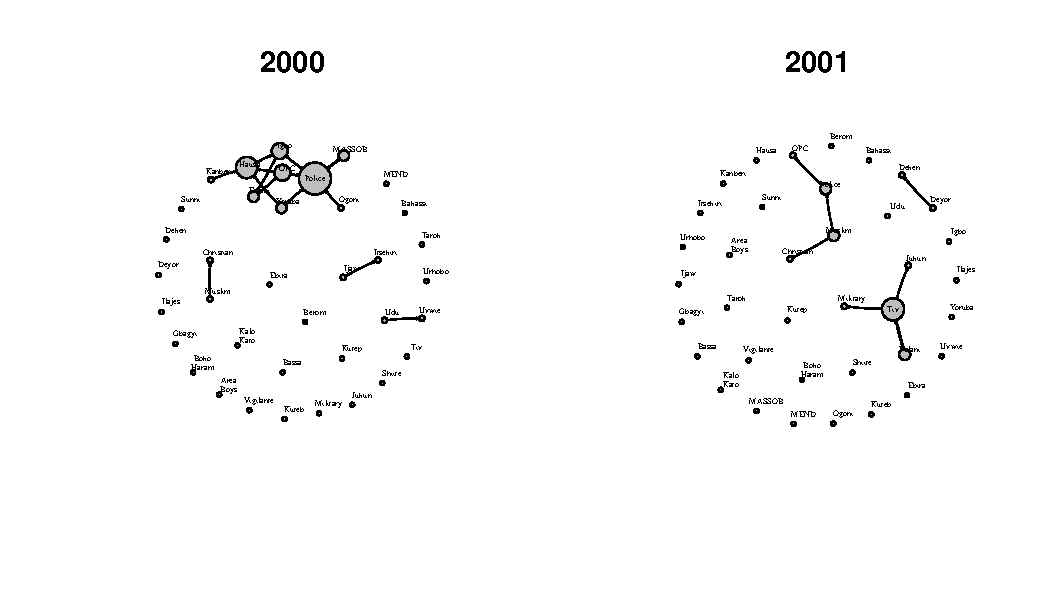
\includegraphics[width=1.1\linewidth]{figure/unnamed-chunk-4-1} 

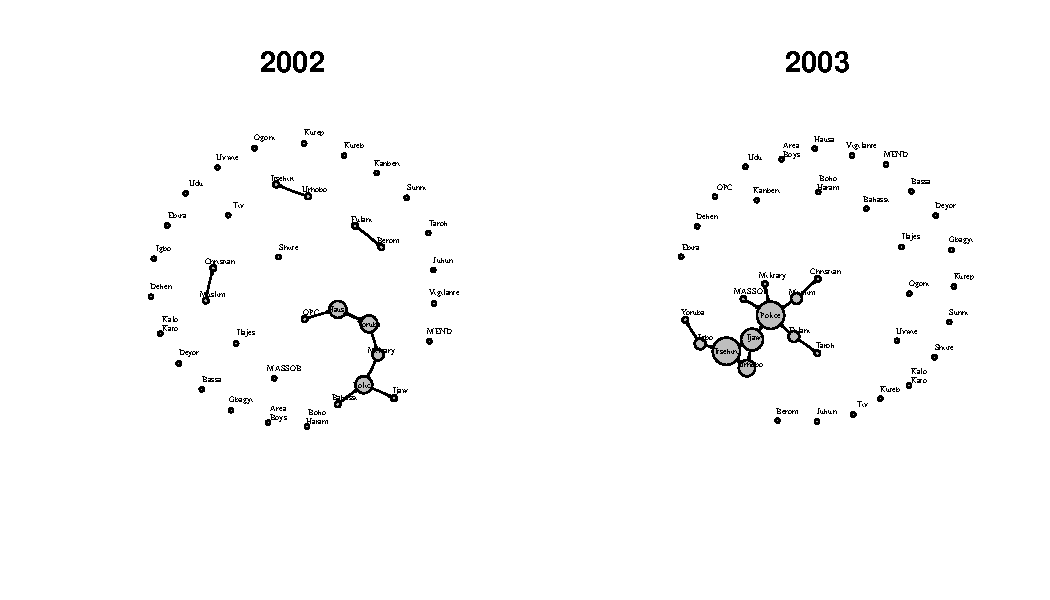
\includegraphics[width=1.1\linewidth]{figure/unnamed-chunk-4-2} 

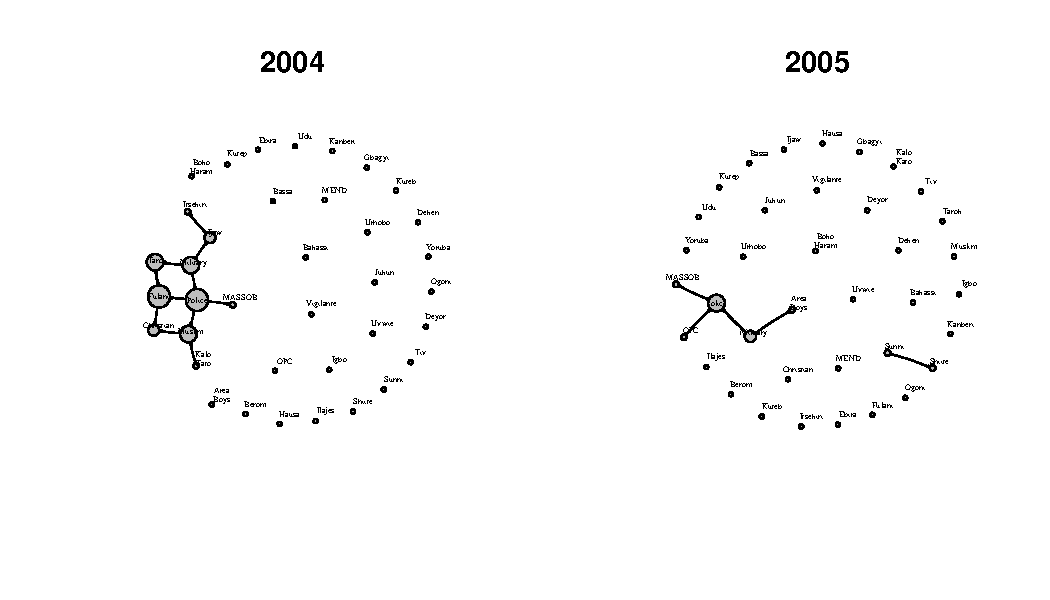
\includegraphics[width=1.1\linewidth]{figure/unnamed-chunk-4-3} 

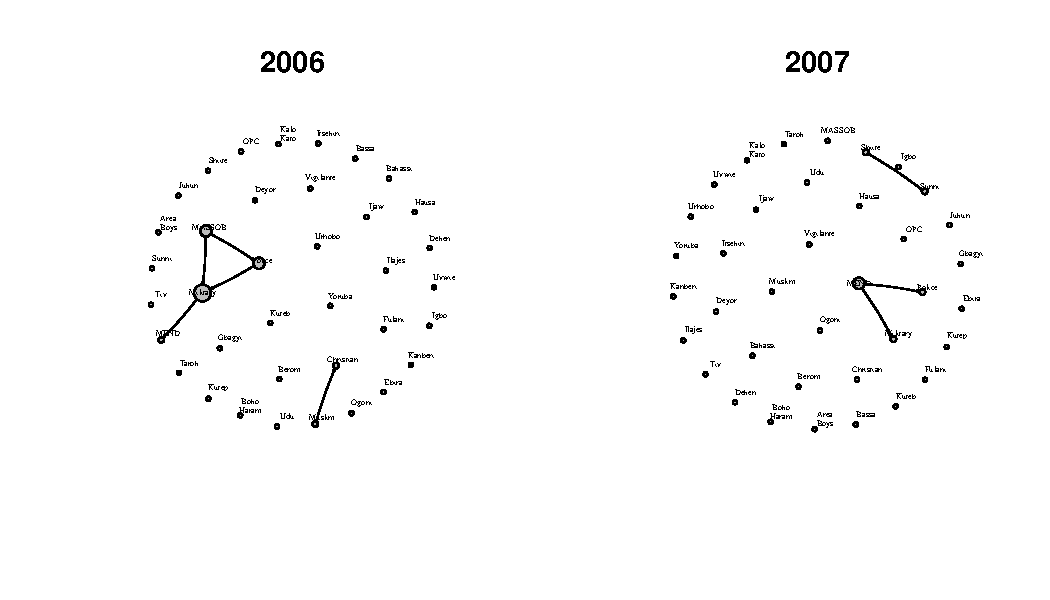
\includegraphics[width=1.1\linewidth]{figure/unnamed-chunk-4-4} 

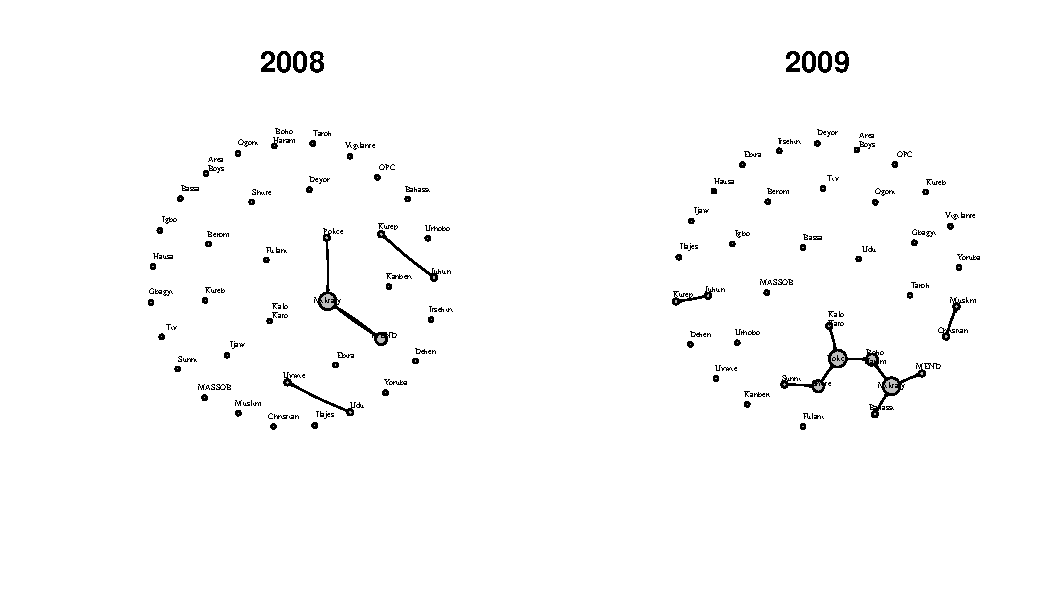
\includegraphics[width=1.1\linewidth]{figure/unnamed-chunk-4-5} 

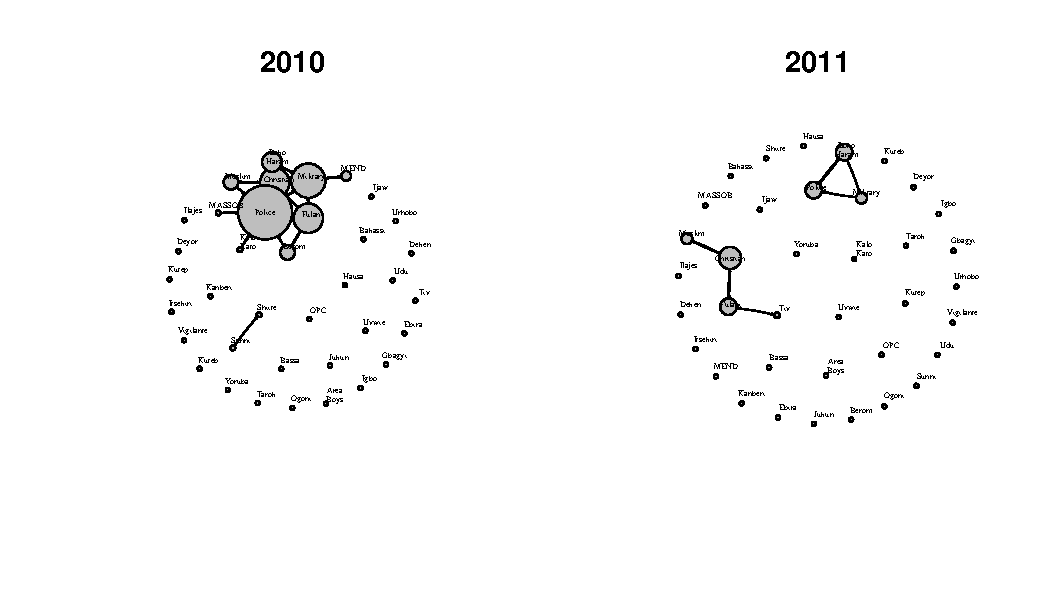
\includegraphics[width=1.1\linewidth]{figure/unnamed-chunk-4-6} 

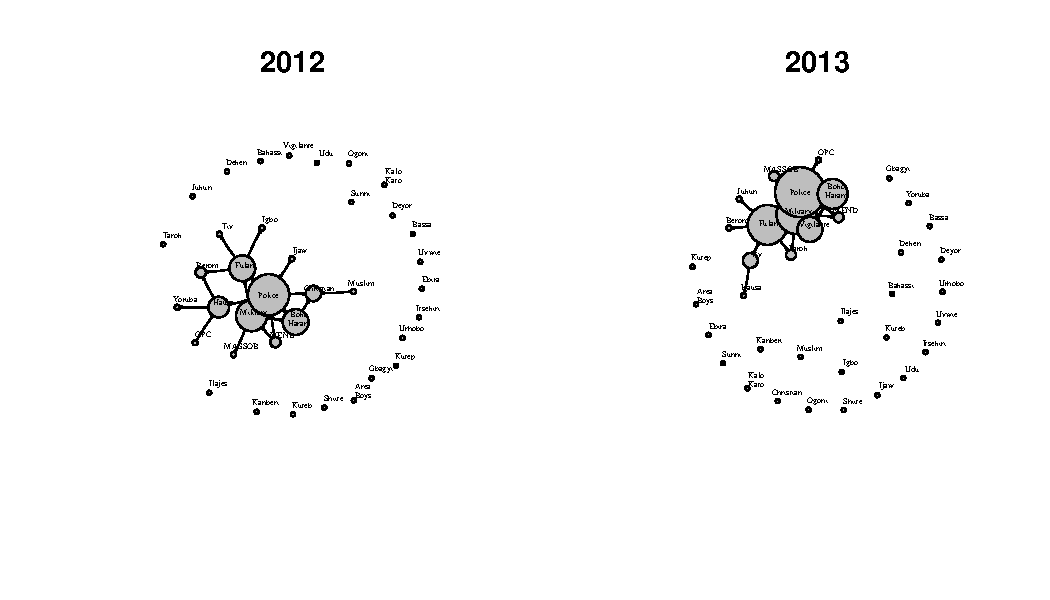
\includegraphics[width=1.1\linewidth]{figure/unnamed-chunk-4-7} 

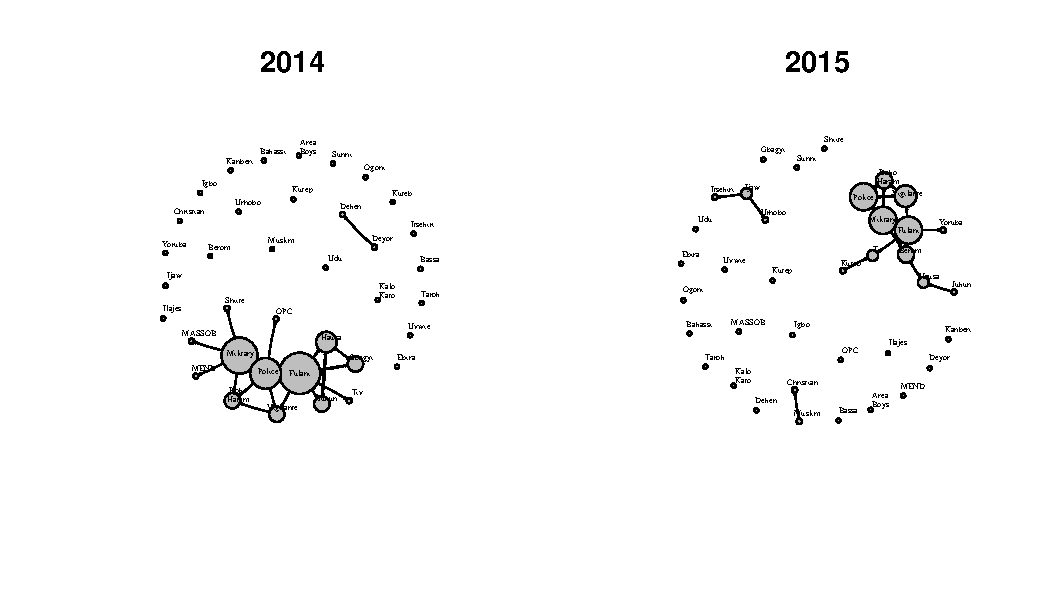
\includegraphics[width=1.1\linewidth]{figure/unnamed-chunk-4-8} 
\begin{kframe}\begin{alltt}
\hlkwd{plot}\hlstd{(nigeriaDyn,} \hlkwc{label} \hlstd{= labels,} \hlkwc{main}\hlstd{=}\hlstr{"All"}\hlstd{,} \hlkwc{label.cex}\hlstd{=}\hlnum{0.5}\hlstd{,} \hlkwc{mode}\hlstd{=}\hlstr{"circle"}\hlstd{,} \hlkwc{vertex.cex}\hlstd{=}\hlkwd{log}\hlstd{(deg_all)}\hlopt{+}\hlnum{1}\hlstd{,}
     \hlkwc{label.col}\hlstd{=}\hlstr{"black"}\hlstd{,} \hlkwc{vertex.col}\hlstd{=}\hlstr{"grey"}\hlstd{,} \hlkwc{edge.col}\hlstd{=}\hlstr{"black"}\hlstd{)}
\end{alltt}
\end{kframe}
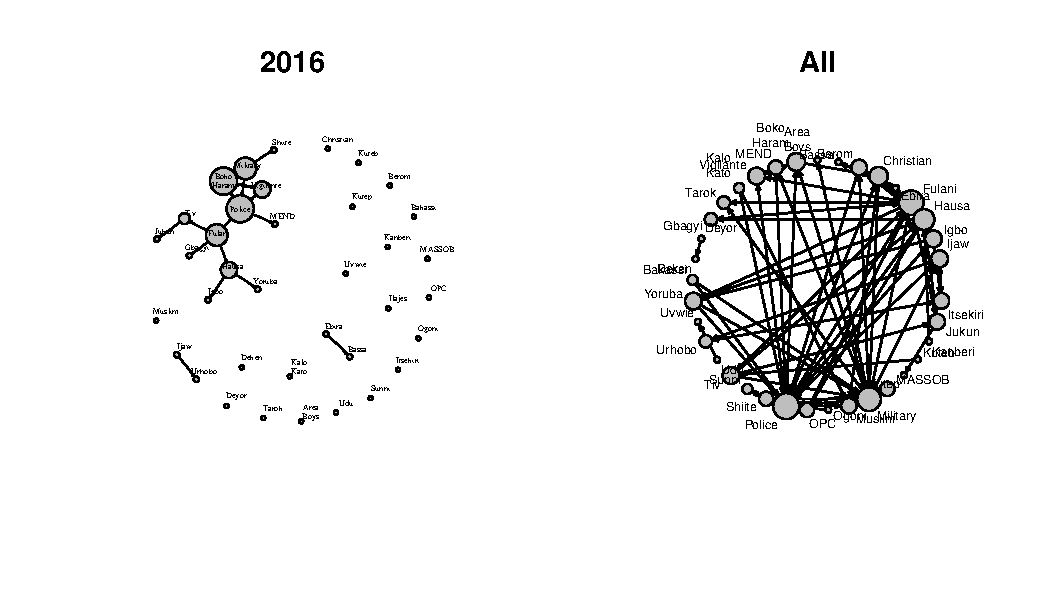
\includegraphics[width=1.1\linewidth]{figure/unnamed-chunk-4-9} 

\end{knitrout}


In the graphs the size of the nodes is based on the global degree and in  most of years the actor with higher degree is the military or the police. By the degree it is clear that Police is the actor more influential, and only the Fulani Militia seems equal influential according to the out-degree measure. Degree seems the best measurment giving that interaction is based on attacks. However if we look at eigenvector centrality still the Police would be the most influential actor. 

Degree seems to be the best way to measure influence when looking year by year as there are many isolated nodes which makes distances or eigenvector centrality less usefull in this case. As seen bellow only in 2001, 2007, 2011 and 2014 the Police or the Military were not the most influential actors. By looking at the in-degree or the receiver, it seems that most of the time the Police was the most influential in most years. Looking at the out-degree the military was the most influential actor.

\begin{knitrout}
\definecolor{shadecolor}{rgb}{0.969, 0.969, 0.969}\color{fgcolor}\begin{kframe}
\begin{alltt}
\hlcom{#Degree}
\hlstd{deg_all} \hlkwb{<-} \hlstd{sna}\hlopt{::}\hlkwd{degree}\hlstd{(nigeriaDyn)}
\hlkwd{paste}\hlstd{(groups[}\hlkwd{which}\hlstd{( deg_all} \hlopt{==} \hlkwd{max}\hlstd{(deg_all) )],} \hlkwc{collapse} \hlstd{=} \hlstr{' '}\hlstd{)}
\end{alltt}
\begin{verbatim}
## [1] "Police\n(Nigeria)"
\end{verbatim}
\begin{alltt}
\hlstd{deg_in_all} \hlkwb{<-} \hlstd{sna}\hlopt{::}\hlkwd{degree}\hlstd{(nigeriaDyn,} \hlkwc{cmode}\hlstd{=}\hlstr{"indegree"}\hlstd{)}
\hlkwd{paste}\hlstd{(groups[}\hlkwd{which}\hlstd{( deg_in_all} \hlopt{==} \hlkwd{max}\hlstd{(deg_in_all) )],} \hlkwc{collapse} \hlstd{=} \hlstr{' '}\hlstd{)}
\end{alltt}
\begin{verbatim}
## [1] "Police\n(Nigeria)"
\end{verbatim}
\begin{alltt}
\hlstd{deg_out_all} \hlkwb{<-} \hlstd{sna}\hlopt{::}\hlkwd{degree}\hlstd{(nigeriaDyn,} \hlkwc{cmode}\hlstd{=}\hlstr{"outdegree"}\hlstd{)}
\hlkwd{paste}\hlstd{(groups[}\hlkwd{which}\hlstd{( deg_out_all} \hlopt{==} \hlkwd{max}\hlstd{(deg_out_all) )],} \hlkwc{collapse} \hlstd{=} \hlstr{' '}\hlstd{)}
\end{alltt}
\begin{verbatim}
## [1] "Fulani\nMilitia Police\n(Nigeria)"
\end{verbatim}
\begin{alltt}
\hlcom{#Eigenvector centrality}
\hlstd{eigen} \hlkwb{<-} \hlstd{sna}\hlopt{::}\hlkwd{evcent}\hlstd{(nigeriaDyn)}
\hlkwd{paste}\hlstd{(groups[}\hlkwd{which}\hlstd{( eigen} \hlopt{==} \hlkwd{max}\hlstd{(eigen) )],} \hlkwc{collapse} \hlstd{=} \hlstr{' '}\hlstd{)}
\end{alltt}
\begin{verbatim}
## [1] "Police\n(Nigeria)"
\end{verbatim}
\begin{alltt}
\hlcom{#Degree year by year}
\hlkwd{as.data.frame}\hlstd{(}\hlkwd{cbind}\hlstd{(years,} \hlstr{"Higher Degree (all)"}\hlstd{=deg_total))}
\end{alltt}
\begin{verbatim}
##    years    Higher Degree (all)
## 1   2000                 Police
## 2   2001                    Tiv
## 3   2002    Hausa Police Yoruba
## 4   2003        Itsekiri Police
## 5   2004          Fulani Police
## 6   2005                 Police
## 7   2006               Military
## 8   2007                   MEND
## 9   2008               Military
## 10  2009        Military Police
## 11  2010                 Police
## 12  2011              Christian
## 13  2012                 Police
## 14  2013                 Police
## 15  2014                 Fulani
## 16  2015 Fulani Military Police
## 17  2016     Police Boko\nHaram
\end{verbatim}
\begin{alltt}
\hlkwd{as.data.frame}\hlstd{(}\hlkwd{cbind}\hlstd{(years,} \hlstr{"Higher Degree (in)"}\hlstd{=deg_in_total))}
\end{alltt}
\begin{verbatim}
##    years                                   Higher Degree (in)
## 1   2000                                               Police
## 2   2001 Christian Fulani Jukun Military OPC Police Tiv Deken
## 3   2002                                         Hausa Police
## 4   2003                                               Police
## 5   2004                        Christian Fulani Muslim Tarok
## 6   2005                                               Police
## 7   2006                                             Military
## 8   2007                                Military Police Sunni
## 9   2008                                             Military
## 10  2009                                   Police Boko\nHaram
## 11  2010                                               Police
## 12  2011                                     Christian Police
## 13  2012                                               Police
## 14  2013                                               Fulani
## 15  2014                                   Fulani Boko\nHaram
## 16  2015                                    Berom Boko\nHaram
## 17  2016                                   Police Boko\nHaram
\end{verbatim}
\begin{alltt}
\hlkwd{as.data.frame}\hlstd{(}\hlkwd{cbind}\hlstd{(years,} \hlstr{"HigherDegree (out)"}\hlstd{=deg_out_total))}
\end{alltt}
\begin{verbatim}
##    years             HigherDegree (out)
## 1   2000                            OPC
## 2   2001                            Tiv
## 3   2002                         Yoruba
## 4   2003                           Ijaw
## 5   2004                Military Police
## 6   2005                       Military
## 7   2006                         MASSOB
## 8   2007                           MEND
## 9   2008 Jukun Military Police Udu MEND
## 10  2009                       Military
## 11  2010                  Fulani Police
## 12  2011   Christian Fulani Boko\nHaram
## 13  2012                Military Police
## 14  2013                         Police
## 15  2014                       Military
## 16  2015                Fulani Military
## 17  2016                         Fulani
\end{verbatim}
\end{kframe}
\end{knitrout}


As seen bellow, k=7 seems to be the best number of groups according to both the AUC (PR) and AUC(ROC).

\begin{knitrout}
\definecolor{shadecolor}{rgb}{0.969, 0.969, 0.969}\color{fgcolor}\begin{kframe}
\begin{alltt}
\hlkwd{set.seed}\hlstd{(}\hlnum{1234}\hlstd{)}

\hlstd{cross} \hlkwb{<-} \hlkwa{function}\hlstd{(}\hlkwc{data}\hlstd{,} \hlkwc{f}\hlstd{=}\hlnum{10}\hlstd{,} \hlkwc{k}\hlstd{=}\hlnum{2}\hlstd{) \{}
    \hlkwd{set.seed}\hlstd{(}\hlnum{1234}\hlstd{)}
    \hlstd{folds} \hlkwb{<-} \hlkwd{createFolds}\hlstd{(groups,} \hlkwc{k}\hlstd{=f,} \hlkwc{returnTrain} \hlstd{= T)}
    \hlstd{tot_pr} \hlkwb{<-} \hlkwd{c}\hlstd{()}
    \hlstd{tot_roc} \hlkwb{<-} \hlkwd{c}\hlstd{()}
    \hlkwa{for} \hlstd{(i} \hlkwa{in} \hlnum{1}\hlopt{:}\hlstd{f) \{}
        \hlstd{nigeriaDyn2} \hlkwb{<-} \hlstd{data}
        \hlstd{network}\hlopt{::}\hlkwd{delete.vertices}\hlstd{(nigeriaDyn2,(}\hlnum{1}\hlopt{:}\hlstd{n)[}\hlopt{-}\hlstd{folds[[i]]])}
        \hlstd{eclusts} \hlkwb{<-} \hlkwd{equiv.clust}\hlstd{(nigeriaDyn2)}
        \hlstd{BlockM} \hlkwb{<-} \hlkwd{blockmodel}\hlstd{(nigeriaDyn2, eclusts,} \hlkwc{k}\hlstd{=k)}
        \hlstd{member} \hlkwb{<-} \hlstd{BlockM}\hlopt{$}\hlstd{block.membership[BlockM}\hlopt{$}\hlstd{order.vec]}

        \hlstd{nigeriaDyn2}\hlopt\hlstr{"member"} \hlkwb{<-} \hlstd{member}
        \hlstd{m} \hlkwb{<-} \hlkwd{btergm}\hlstd{(}\hlkwd{as.network.networkDynamic}\hlstd{(nigeriaDyn2)} \hlopt{~} \hlstd{edges} \hlopt{+}
                             \hlkwd{gwesp}\hlstd{(}\hlnum{.5}\hlstd{,} \hlkwc{fixed} \hlstd{=} \hlnum{TRUE}\hlstd{)} \hlopt{+} \hlkwd{nodecov}\hlstd{(}\hlstr{"member"}\hlstd{))}
        \hlcom{#probs <- edgeprob(m)}

        \hlstd{g} \hlkwb{<-} \hlkwd{gof}\hlstd{(m,} \hlkwc{statistics} \hlstd{= rocpr,} \hlkwc{nsim} \hlstd{=} \hlnum{50}\hlstd{)}
        \hlstd{tot_pr} \hlkwb{<-} \hlkwd{c}\hlstd{(tot_pr, g}\hlopt{$}\hlstd{`Tie prediction`}\hlopt{$}\hlstd{auc.roc)}
        \hlstd{tot_roc} \hlkwb{<-} \hlkwd{c}\hlstd{(tot_pr, g}\hlopt{$}\hlstd{`Tie prediction`}\hlopt{$}\hlstd{auc.pr)}



    \hlstd{\}}
    \hlkwd{return}\hlstd{(}\hlkwd{list}\hlstd{(}\hlkwc{PR}\hlstd{=}\hlkwd{mean}\hlstd{(tot_pr),} \hlkwc{ROC}\hlstd{=}\hlkwd{mean}\hlstd{(tot_roc)))}
\hlstd{\}}


\hlstd{pr_results} \hlkwb{<-} \hlkwd{c}\hlstd{()}
\hlstd{roc_results} \hlkwb{<-} \hlkwd{c}\hlstd{()}
\hlkwa{for} \hlstd{(k} \hlkwa{in} \hlnum{2}\hlopt{:}\hlnum{10}\hlstd{) \{}
  \hlstd{cross_results} \hlkwb{<-} \hlkwd{cross}\hlstd{(nigeriaDyn,} \hlkwc{k}\hlstd{=k)}
  \hlstd{pr_results} \hlkwb{<-} \hlkwd{c}\hlstd{(pr_results, cross_results}\hlopt{$}\hlstd{PR)}
  \hlstd{roc_results} \hlkwb{<-} \hlkwd{c}\hlstd{(roc_results, cross_results}\hlopt{$}\hlstd{ROC)}
\hlstd{\}}
\hlkwd{data.frame}\hlstd{(}\hlkwc{k}\hlstd{=}\hlnum{2}\hlopt{:}\hlnum{10}\hlstd{,}\hlkwc{PR}\hlstd{=pr_results,} \hlkwc{ROC}\hlstd{=roc_results)}
\end{alltt}
\begin{verbatim}
##    k        PR       ROC
## 1  2 0.5235649 0.4809065
## 2  3 0.5371697 0.4923879
## 3  4 0.5502108 0.5044855
## 4  5 0.5399445 0.4963676
## 5  6 0.5561239 0.5117770
## 6  7 0.5787657 0.5327670
## 7  8 0.5518961 0.5065237
## 8  9 0.5367710 0.4937206
## 9 10 0.5307155 0.4878298
\end{verbatim}
\end{kframe}
\end{knitrout}

\begin{knitrout}
\definecolor{shadecolor}{rgb}{0.969, 0.969, 0.969}\color{fgcolor}\begin{kframe}
\begin{alltt}
\hlstd{eclusts} \hlkwb{<-} \hlkwd{equiv.clust}\hlstd{(nigeriaDyn)}
\hlstd{BlockM} \hlkwb{<-} \hlkwd{blockmodel}\hlstd{(nigeriaDyn, eclusts,} \hlkwc{k}\hlstd{=}\hlnum{7}\hlstd{)}
\hlstd{member_or} \hlkwb{<-} \hlstd{BlockM}\hlopt{$}\hlstd{block.membership[BlockM}\hlopt{$}\hlstd{order.vec]}

\hlstd{nigeriaDyn}\hlopt\hlstr{"member"} \hlkwb{<-} \hlstd{member_or}
\hlcom{#nigeriaDyn %v% "member"}
\hlstd{nigeriaDyn} \hlopt \hlstr{"col"} \hlkwb{<-} \hlkwd{c}\hlstd{(}\hlstr{"gray70"}\hlstd{,} \hlstr{"tomato"}\hlstd{,} \hlstr{"gold"}\hlstd{,} \hlstr{"yellow"}\hlstd{,} \hlstr{"blue"}\hlstd{,} \hlstr{"red"}\hlstd{,} \hlstr{"orange"}\hlstd{)[nigeriaDyn} \hlopt \hlstr{"member"}\hlstd{]}

\hlkwd{plot}\hlstd{(nigeriaDyn,} \hlkwc{label} \hlstd{= labels,} \hlkwc{label.cex}\hlstd{=}\hlnum{0.5}\hlstd{,} \hlkwc{mode}\hlstd{=}\hlstr{"circle"}\hlstd{,} \hlkwc{vertex.cex}\hlstd{=}\hlkwd{log}\hlstd{(deg_all)}\hlopt{+}\hlnum{1}\hlstd{,}
     \hlkwc{label.col}\hlstd{=}\hlstr{"black"}\hlstd{,} \hlkwc{vertex.col}\hlstd{=}\hlstr{"col"}\hlstd{,} \hlkwc{vertex.border}\hlstd{=}\hlstr{"col"}\hlstd{,} \hlkwc{edge.col}\hlstd{=}\hlstr{"black"}\hlstd{)}
\end{alltt}
\end{kframe}
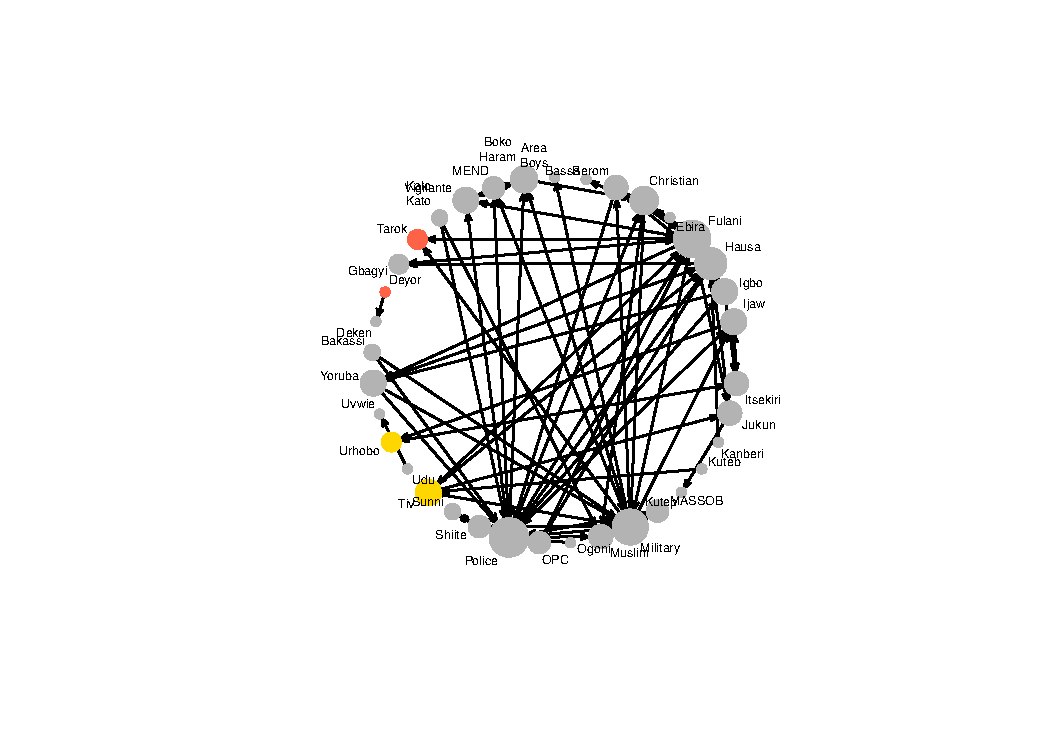
\includegraphics[width=1.1\linewidth]{figure/unnamed-chunk-7-1} 

\end{knitrout}

The first logical hypothesis would be that if a reciprocal tie is present then the odds of a tie would be higher. If an actor attacks, the odd of a retaliation should be higher. For this, it is important to include the term mutual in the ERGM. Including an attribute variable of whether the actor is the Police or the Military may be another important variable to include. It should be expected no attacks between them. Another hypothesis could be that the more an actor has 2 stars the more likely that actor would attack others. This may be important given that two popular actors are in consideration, the police and the military. If two actors attack another third, it should be more likely for them not to attack themselves. For this, it is included the term triangles. And we may discount each additional tie by including the term gwidegree.

As expected the coefficient for mutual is positive so it is very likely retaliation among actors. The strong negative coefficient for the group-homophily term shows that the police and the military do not attack themselves. The triangle couldn't be estimated because there are few triangles in this network. 


\begin{knitrout}
\definecolor{shadecolor}{rgb}{0.969, 0.969, 0.969}\color{fgcolor}\begin{kframe}
\begin{alltt}
\hlstd{nigeria1} \hlkwb{<-} \hlstd{nigerialist[[}\hlnum{1}\hlstd{]]}
\hlstd{nigeria1}\hlopt\hlstr{"gov"} \hlkwb{<-} \hlkwd{ifelse}\hlstd{(groups}\hlopt{==}\hlstr{"Police\textbackslash{}n(Nigeria)"}\hlopt{|} \hlstd{groups}\hlopt{==}\hlstr{"Military\textbackslash{}n(Nigeria)"}\hlstd{,}\hlnum{1}\hlstd{,}\hlnum{0}\hlstd{)}
\hlstd{m} \hlkwb{=} \hlkwd{ergm}\hlstd{(nigeria1} \hlopt{~} \hlstd{edges} \hlopt{+} \hlstd{mutual}\hlopt{+} \hlkwd{nodematch}\hlstd{(}\hlstr{"gov"}\hlstd{)} \hlopt{+} \hlkwd{istar}\hlstd{(}\hlnum{2}\hlstd{)}\hlopt{+} \hlstd{triangle}\hlopt{+}\hlkwd{gwidegree}\hlstd{(}\hlkwc{decay} \hlstd{=} \hlnum{0.5}\hlstd{,} \hlkwc{fixed} \hlstd{=} \hlnum{TRUE}\hlstd{))}
\hlkwd{summary}\hlstd{(m)}
\end{alltt}
\begin{verbatim}
## 
## ==========================
## Summary of model fit
## ==========================
## 
## Formula:   nigeria1 ~ edges + mutual + nodematch("gov") + istar(2) + triangle + 
##     gwidegree(decay = 0.5, fixed = TRUE)
## 
## Iterations:  2 out of 20 
## 
## Monte Carlo MLE Results:
##               Estimate Std. Error MCMC % p-value    
## edges          0.04503    2.62266      0  0.9863    
## mutual         2.37950    1.11987      0  0.0338 *  
## nodematch.gov -1.09842    0.47448      0  0.0208 *  
## istar2        -0.73410    0.96313      0  0.4461    
## triangle          -Inf    0.00000      0  <1e-04 ***
## gwidegree     -4.80796    2.85555      0  0.0925 .  
## ---
## Signif. codes:  0 '***' 0.001 '**' 0.01 '*' 0.05 '.' 0.1 ' ' 1
## 
##      Null Deviance: 1847  on 1332  degrees of freedom
##  Residual Deviance:  NaN  on 1326  degrees of freedom
##  
## AIC: NaN    BIC: NaN    (Smaller is better.) 
## 
##  Warning: The following terms have infinite coefficient estimates:
##   triangle
\end{verbatim}
\end{kframe}
\end{knitrout}

Bellow it is shown the MCM diagnostics, it seems well-mixed and with stationary chains. 

\begin{knitrout}
\definecolor{shadecolor}{rgb}{0.969, 0.969, 0.969}\color{fgcolor}\begin{kframe}
\begin{alltt}
\hlkwd{mcmc.diagnostics}\hlstd{(m)}
\end{alltt}
\begin{verbatim}
## Sample statistics summary:
## 
## Iterations = 16384:4209664
## Thinning interval = 1024 
## Number of chains = 1 
## Sample size per chain = 4096 
## 
## 1. Empirical mean and standard deviation for each variable,
##    plus standard error of the mean:
## 
##                  Mean    SD Naive SE Time-series SE
## edges          0.1099 5.627  0.08792        0.09474
## mutual         0.2222 1.200  0.01875        0.02110
## nodematch.gov  1.3191 4.415  0.06898        0.06898
## istar2        -0.6309 6.537  0.10214        0.11122
## gwidegree      0.3317 3.359  0.05248        0.05565
## 
## 2. Quantiles for each variable:
## 
##                  2.5%    25%     50%   75%  97.5%
## edges         -10.000 -4.000  0.0000 4.000 12.000
## mutual         -1.000 -1.000  0.0000 1.000  3.000
## nodematch.gov  -6.000 -2.000  1.0000 4.000 11.000
## istar2        -10.000 -6.000 -2.0000 3.000 15.000
## gwidegree      -5.848 -2.061  0.1548 2.571  7.168
## 
## 
## Sample statistics cross-correlations:
##                   edges    mutual nodematch.gov    istar2 gwidegree
## edges         1.0000000 0.6451016     0.8536075 0.8567962 0.9430548
## mutual        0.6451016 1.0000000     0.4661134 0.5527570 0.6085496
## nodematch.gov 0.8536075 0.4661134     1.0000000 0.6453335 0.8515740
## istar2        0.8567962 0.5527570     0.6453335 1.0000000 0.6452543
## gwidegree     0.9430548 0.6085496     0.8515740 0.6452543 1.0000000
## 
## Sample statistics auto-correlation:
## Chain 1 
##                  edges       mutual nodematch.gov       istar2
## Lag 0     1.0000000000  1.000000000    1.00000000  1.000000000
## Lag 1024  0.0745023118  0.117637222    0.01497454  0.084838496
## Lag 2048 -0.0016078931  0.012019314   -0.01324165 -0.000231895
## Lag 3072 -0.0112532712 -0.011026355   -0.01067052 -0.002124739
## Lag 4096  0.0002175683  0.024690048   -0.02199732  0.019639235
## Lag 5120 -0.0233379084 -0.008498069   -0.02003264 -0.022915736
##              gwidegree
## Lag 0     1.0000000000
## Lag 1024  0.0584582952
## Lag 2048 -0.0002112205
## Lag 3072 -0.0090114816
## Lag 4096 -0.0135061043
## Lag 5120 -0.0211166244
## 
## Sample statistics burn-in diagnostic (Geweke):
## Chain 1 
## 
## Fraction in 1st window = 0.1
## Fraction in 2nd window = 0.5 
## 
##         edges        mutual nodematch.gov        istar2     gwidegree 
##       0.12778      -0.45316      -0.39710       0.28642      -0.01315 
## 
## Individual P-values (lower = worse):
##         edges        mutual nodematch.gov        istar2     gwidegree 
##     0.8983269     0.6504361     0.6912923     0.7745529     0.9895095 
## Joint P-value (lower = worse):  0.8791296 .
\end{verbatim}
\end{kframe}
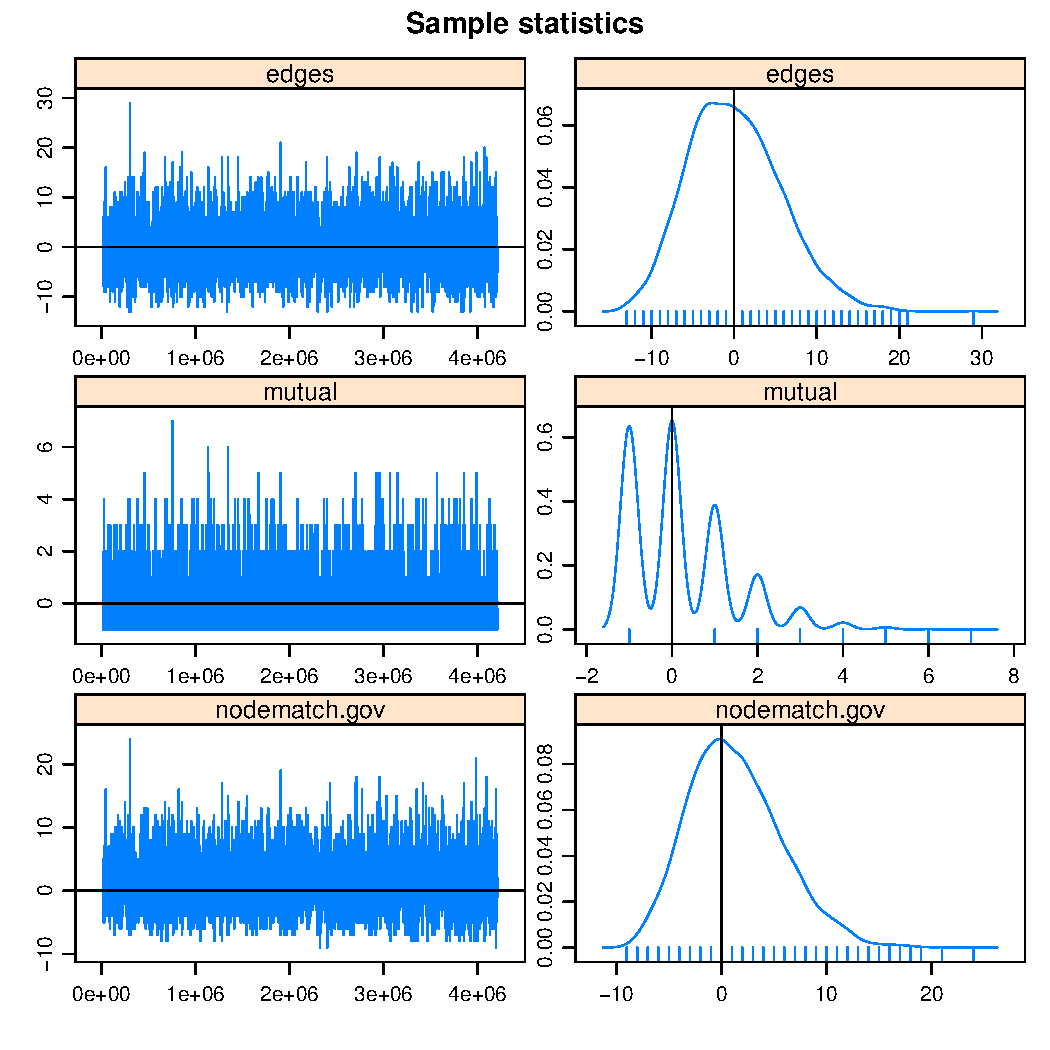
\includegraphics[width=\maxwidth]{figure/unnamed-chunk-9-1} 

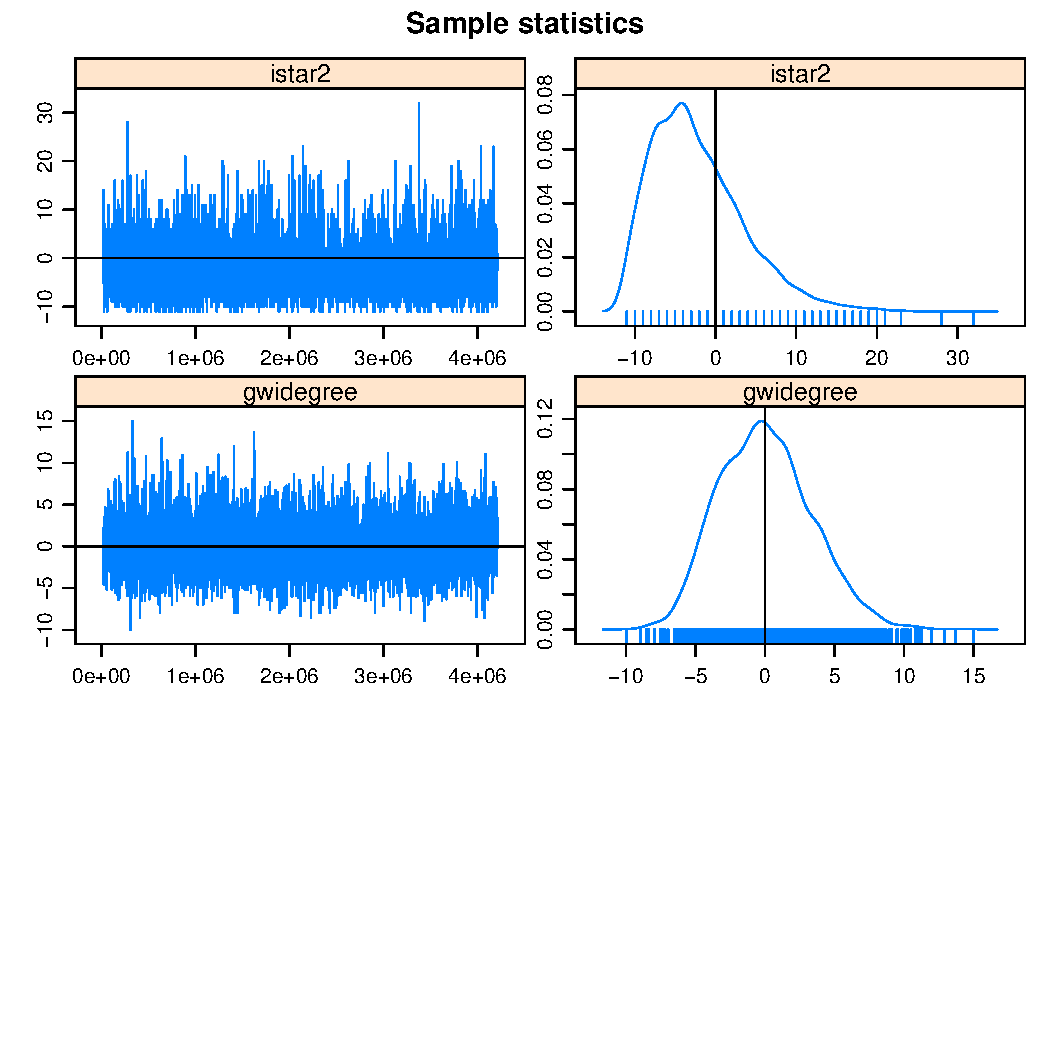
\includegraphics[width=\maxwidth]{figure/unnamed-chunk-9-2} 
\begin{kframe}\begin{verbatim}
## 
## MCMC diagnostics shown here are from the last round of simulation, prior to computation of final parameter estimates. Because the final estimates are refinements of those used for this simulation run, these diagnostics may understate model performance. To directly assess the performance of the final model on in-model statistics, please use the GOF command: gof(ergmFitObject, GOF=~model).
\end{verbatim}
\end{kframe}
\end{knitrout}




\end{document}
